\batchmode
\documentclass[twoside]{article}

% Packages required by doxygen
\usepackage{fixltx2e}
\usepackage{calc}
\usepackage{doxygen}
\usepackage[export]{adjustbox} % also loads graphicx
\usepackage{graphicx}
\usepackage[utf8]{inputenc}
\usepackage{makeidx}
\usepackage{multicol}
\usepackage{multirow}
\PassOptionsToPackage{warn}{textcomp}
\usepackage{textcomp}
\usepackage[nointegrals]{wasysym}
\usepackage[table]{xcolor}

% Font selection
\usepackage[T1]{fontenc}
\usepackage[scaled=.90]{helvet}
\usepackage{courier}
\usepackage{amssymb}
\usepackage{sectsty}
\renewcommand{\familydefault}{\sfdefault}
\allsectionsfont{%
  \fontseries{bc}\selectfont%
  \color{darkgray}%
}
\renewcommand{\DoxyLabelFont}{%
  \fontseries{bc}\selectfont%
  \color{darkgray}%
}
\newcommand{\+}{\discretionary{\mbox{\scriptsize$\hookleftarrow$}}{}{}}

% Page & text layout
\usepackage{geometry}
\geometry{%
  a4paper,%
  top=2.5cm,%
  bottom=2.5cm,%
  left=2.5cm,%
  right=2.5cm%
}
\tolerance=750
\hfuzz=15pt
\hbadness=750
\setlength{\emergencystretch}{15pt}
\setlength{\parindent}{0cm}
\setlength{\parskip}{3ex plus 2ex minus 2ex}
\makeatletter
\renewcommand{\paragraph}{%
  \@startsection{paragraph}{4}{0ex}{-1.0ex}{1.0ex}{%
    \normalfont\normalsize\bfseries\SS@parafont%
  }%
}
\renewcommand{\subparagraph}{%
  \@startsection{subparagraph}{5}{0ex}{-1.0ex}{1.0ex}{%
    \normalfont\normalsize\bfseries\SS@subparafont%
  }%
}
\makeatother

% Headers & footers
\usepackage{fancyhdr}
\pagestyle{fancyplain}
\fancyhead[LE]{\fancyplain{}{\bfseries\thepage}}
\fancyhead[CE]{\fancyplain{}{}}
\fancyhead[RE]{\fancyplain{}{\bfseries\leftmark}}
\fancyhead[LO]{\fancyplain{}{\bfseries\rightmark}}
\fancyhead[CO]{\fancyplain{}{}}
\fancyhead[RO]{\fancyplain{}{\bfseries\thepage}}
\fancyfoot[LE]{\fancyplain{}{}}
\fancyfoot[CE]{\fancyplain{}{}}
\fancyfoot[RE]{\fancyplain{}{\bfseries\scriptsize Generated by Doxygen }}
\fancyfoot[LO]{\fancyplain{}{\bfseries\scriptsize Generated by Doxygen }}
\fancyfoot[CO]{\fancyplain{}{}}
\fancyfoot[RO]{\fancyplain{}{}}
\renewcommand{\footrulewidth}{0.4pt}
\renewcommand{\sectionmark}[1]{%
  \markright{\thesection\ #1}%
}

% Indices & bibliography
\usepackage{natbib}
\usepackage[titles]{tocloft}
\setcounter{tocdepth}{3}
\setcounter{secnumdepth}{5}
\makeindex

% Packages requested by user
\usepackage{C:/Data/Tom/Research/Raedler/mRNA-Helmholtz/Tom/GenSSI/Docu/config/latexextras}

% Hyperlinks (required, but should be loaded last)
\usepackage{ifpdf}
\ifpdf
  \usepackage[pdftex,pagebackref=true]{hyperref}
\else
  \usepackage[ps2pdf,pagebackref=true]{hyperref}
\fi
\hypersetup{%
  colorlinks=true,%
  linkcolor=blue,%
  citecolor=blue,%
  unicode%
}

% Custom commands
\newcommand{\clearemptydoublepage}{%
  \newpage{\pagestyle{empty}\cleardoublepage}%
}

\usepackage{caption}
\captionsetup{labelsep=space,justification=centering,font={bf},singlelinecheck=off,skip=4pt,position=top}

%===== C O N T E N T S =====

\begin{document}

% Titlepage & ToC
\hypersetup{pageanchor=false,
             bookmarksnumbered=true,
             pdfencoding=unicode
            }
\pagenumbering{roman}
\begin{titlepage}
\vspace*{7cm}
\begin{center}%
{\Large Gen\+S\+SI \\[1ex]\large 2016-\/02-\/19 }\\
\vspace*{1cm}
{\large Generated by Doxygen 1.8.11}\\
\end{center}
\end{titlepage}
\tableofcontents
\pagenumbering{arabic}
\hypersetup{pageanchor=true}

%--- Begin generated contents ---
\section{Gen\+S\+SI 2.0 General Documentation}
\label{index}\hypertarget{index}{}\hypertarget{index_intro}{}\subsection{Introduction}\label{index_intro}
Gen\+S\+SI is a Matlab implementation of generating series for structural identifiability as defined in


\begin{DoxyItemize}
\item Chiş, O.-\/T., Banga, J.\+R. and Balsa-\/\+Canto, E. (2011) Structural Identifiability of Systems Biology Models\+: A Critical Comparison of Methods, P\+LoS O\+NE, 6, e27755.
\item Chiş, O., Banga, J.\+R. and Balsa-\/\+Canto, E. (2011) Gen\+S\+SI\+: a software toolbox for structural identifiability analysis of biological models, Bioinformatics, 27, 2610-\/2611.
\end{DoxyItemize}

With Gen\+S\+SI, the user can specify differential equation models in terms of symbolic variables in Matlab and then analyze the models to determine which parameters are globally or locally identifiable. In addition, there are some utilities for converting models to polynomial form, or to or from A\+M\+I\+CI format.\hypertarget{index_download}{}\subsection{Availability}\label{index_download}
The sources for Gen\+S\+SI are accessible as
\begin{DoxyItemize}
\item Source \href{https://github.com/thomassligon/GenSSI/tarball/master}{\tt tarball}
\item Source \href{https://github.com/thomassligon/GenSSI/zipball/master}{\tt zipball}
\item Git repository on \href{https://github.com/thomassligon/GenSSI}{\tt github}
\end{DoxyItemize}

Once you\textquotesingle{}ve obtained your copy check out the \hyperlink{index_install}{Installation}\hypertarget{index_git}{}\subsubsection{Obtaining Gen\+S\+S\+I via the Git versioning system}\label{index_git}
In order to always stay up to date with the latest Gen\+S\+SI versions, simply pull it from our Git repository and recompile it when a new release is available. For more information about Git checkout their \href{http://git-scm.com/}{\tt website}

The Git repository can currently be found at \href{https://github.com/thomassligon/GenSSI}{\tt https\+://github.\+com/thomassligon/\+Gen\+S\+SI} and a direct clone is possible via 
\begin{DoxyCode}
git clone https:\textcolor{comment}{//github.com/thomassligon/GenSSI.git GenSSI }
\end{DoxyCode}
\hypertarget{index_GenSSI}{}\subsubsection{License Conditions}\label{index_GenSSI}
This software is available under the \href{http://www.opensource.org/licenses/bsd-license.php}{\tt B\+SD license}

Copyright (c) 2016, Oana-\/\+Teodora Chiş, Julio R. Banga, Eva Balsa-\/\+Canto, Thomas S. Ligon, Fabian Fröhlich and Jan Hasenauer. All rights reserved.

Redistribution and use in source and binary forms, with or without modification, are permitted provided that the following conditions are met\+:
\begin{DoxyItemize}
\item Redistributions of source code must retain the above copyright notice, this list of conditions and the following disclaimer.
\item Redistributions in binary form must reproduce the above copyright notice, this list of conditions and the following disclaimer in the documentation and/or other materials provided with the distribution.
\end{DoxyItemize}

T\+H\+IS S\+O\+F\+T\+W\+A\+RE IS P\+R\+O\+V\+I\+D\+ED BY T\+HE C\+O\+P\+Y\+R\+I\+G\+HT H\+O\+L\+D\+E\+RS A\+ND C\+O\+N\+T\+R\+I\+B\+U\+T\+O\+RS \char`\"{}\+A\+S I\+S\char`\"{} A\+ND A\+NY E\+X\+P\+R\+E\+SS OR I\+M\+P\+L\+I\+ED W\+A\+R\+R\+A\+N\+T\+I\+ES, I\+N\+C\+L\+U\+D\+I\+NG, B\+UT N\+OT L\+I\+M\+I\+T\+ED TO, T\+HE I\+M\+P\+L\+I\+ED W\+A\+R\+R\+A\+N\+T\+I\+ES OF M\+E\+R\+C\+H\+A\+N\+T\+A\+B\+I\+L\+I\+TY A\+ND F\+I\+T\+N\+E\+SS F\+OR A P\+A\+R\+T\+I\+C\+U\+L\+AR P\+U\+R\+P\+O\+SE A\+RE D\+I\+S\+C\+L\+A\+I\+M\+ED. IN NO E\+V\+E\+NT S\+H\+A\+LL T\+HE C\+O\+P\+Y\+R\+I\+G\+HT H\+O\+L\+D\+ER OR C\+O\+N\+T\+R\+I\+B\+U\+T\+O\+RS BE L\+I\+A\+B\+LE F\+OR A\+NY D\+I\+R\+E\+CT, I\+N\+D\+I\+R\+E\+CT, I\+N\+C\+I\+D\+E\+N\+T\+AL, S\+P\+E\+C\+I\+AL, E\+X\+E\+M\+P\+L\+A\+RY, OR C\+O\+N\+S\+E\+Q\+U\+E\+N\+T\+I\+AL D\+A\+M\+A\+G\+ES (I\+N\+C\+L\+U\+D\+I\+NG, B\+UT N\+OT L\+I\+M\+I\+T\+ED TO, P\+R\+O\+C\+U\+R\+E\+M\+E\+NT OF S\+U\+B\+S\+T\+I\+T\+U\+TE G\+O\+O\+DS OR S\+E\+R\+V\+I\+C\+ES; L\+O\+SS OF U\+SE, D\+A\+TA, OR P\+R\+O\+F\+I\+TS; OR B\+U\+S\+I\+N\+E\+SS I\+N\+T\+E\+R\+R\+U\+P\+T\+I\+ON) H\+O\+W\+E\+V\+ER C\+A\+U\+S\+ED A\+ND ON A\+NY T\+H\+E\+O\+RY OF L\+I\+A\+B\+I\+L\+I\+TY, W\+H\+E\+T\+H\+ER IN C\+O\+N\+T\+R\+A\+CT, S\+T\+R\+I\+CT L\+I\+A\+B\+I\+L\+I\+TY, OR T\+O\+RT (I\+N\+C\+L\+U\+D\+I\+NG N\+E\+G\+L\+I\+G\+E\+N\+CE OR O\+T\+H\+E\+R\+W\+I\+SE) A\+R\+I\+S\+I\+NG IN A\+NY W\+AY O\+UT OF T\+HE U\+SE OF T\+H\+IS S\+O\+F\+T\+W\+A\+RE, E\+V\+EN IF A\+D\+V\+I\+S\+ED OF T\+HE P\+O\+S\+S\+I\+B\+I\+L\+I\+TY OF S\+U\+CH D\+A\+M\+A\+GE.\hypertarget{index_install}{}\subsection{Installation}\label{index_install}
If Gen\+S\+SI was downloaded as a zip, it needs to be unpacked in a convenient directory. If Gen\+S\+SI was obtained via cloning of the git repository, no further unpacking is necessary.

Models are generally stored in 
\begin{DoxyCode}
GenSSI/Examples 
\end{DoxyCode}
 but Gen\+S\+SI should be able to find them in any directory that is is the Matlab path.

When a model is analyzed Gen\+S\+SI stores the results in 
\begin{DoxyCode}
GenSSI/Results 
\end{DoxyCode}


To use Gen\+S\+SI, start Matlab and add the Gen\+S\+SI direcory to the Matlab path. To add all toolbox directories to the Matlab path, execute the Matlab script 
\begin{DoxyCode}
\hyperlink{genssi_startup_8m_addcff165cb4278db5bc6df9f60bff280}{genssiStartup}.m 
\end{DoxyCode}
 To store the installation for further Matlab session, the path can be saved via 
\begin{DoxyCode}
savepath 
\end{DoxyCode}
 
\section{Model Definition \& Simulation}
\label{def_simu}
\hypertarget{def_simu}{}
In the following we will give a detailed overview how to specify models in Gen\+S\+SI and how to call the code for analyzing the model. We use the Goodwin oscillator as an example.\hypertarget{def_simu_definition}{}\subsection{Model Definition}\label{def_simu_definition}
This manual will guide the user to specify models in Matlab. For example implementations, see the models in the example directory.\hypertarget{def_simu_header}{}\subsubsection{Header}\label{def_simu_header}
The model definition needs to be defined as a function which returns a struct with all symbolic definitions and options.


\begin{DoxyCode}
\textcolor{keyword}{function} [model] = Goodwin() 
\end{DoxyCode}
\hypertarget{def_simu_name}{}\subsubsection{Name}\label{def_simu_name}
Give the model a name.


\begin{DoxyCode}
model.Name = \textcolor{stringliteral}{'Goodwin'}; 
\end{DoxyCode}
\hypertarget{def_simu_derivatives}{}\subsubsection{Derivatives}\label{def_simu_derivatives}
Set the number of derivatives to be calculated.


\begin{DoxyCode}
model.Nder = 8; 
\end{DoxyCode}
\hypertarget{def_simu_states}{}\subsubsection{States}\label{def_simu_states}
Create the respective symbolic variables. The name of the symbolic variable can be chosen arbitrarily.


\begin{DoxyCode}
syms x1 x2 x3 
\end{DoxyCode}


Create the state vector containing all states\+:


\begin{DoxyCode}
model.X = [x1 x2 x3]; 
\end{DoxyCode}


Define the number of states.


\begin{DoxyCode}
model.Neq = 3; 
\end{DoxyCode}
\hypertarget{def_simu_parameters}{}\subsubsection{Parameters}\label{def_simu_parameters}
Create the respective symbolic variables. The name of the symbolic variable can be chosen arbitrarily.


\begin{DoxyCode}
syms p1 p2 p3 p4 p5 p6 p7 p8 
\end{DoxyCode}


Create the parameters vector of parameters to be considered for identifiability.


\begin{DoxyCode}
model.Par = [p1 p2 p3 p4 p5 p6 p7 p8]; 
\end{DoxyCode}


Specify the number of parameters to be considered for identifiability.


\begin{DoxyCode}
model.Npar = 8; 
\end{DoxyCode}
\hypertarget{def_simu_equtions}{}\subsubsection{Equations}\label{def_simu_equtions}
Define the equations of the model.


\begin{DoxyCode}
A1 = -p4*x1+p1/(p2+x3^p3);
A2 = p5*x1-p6*x2;
A3 = p7*x2-p8*x3;
model.F=[A1 A2 A3];
\end{DoxyCode}
\hypertarget{def_simu_controls}{}\subsubsection{Controls}\label{def_simu_controls}
Define the controls.


\begin{DoxyCode}
g1=0;
g2=0;
g3=0;
model.G=[g1 g2 Ag3];
\end{DoxyCode}


Define the number of controls.


\begin{DoxyCode}
model.Noc = 0; 
\end{DoxyCode}


Note that the length of the control vector should match the number of states, even if there are fewer controls.\hypertarget{def_simu_obserables}{}\subsubsection{Observables}\label{def_simu_obserables}
Define the observables.


\begin{DoxyCode}
h1 = x1;
h2 = x2;
h3 = x3;
model.H = [h1 h2 h3];
\end{DoxyCode}


Define the number of obserables.


\begin{DoxyCode}
model.Nobs = 1; 
\end{DoxyCode}
\hypertarget{def_simu_ic}{}\subsubsection{Initial Conditions}\label{def_simu_ic}
Define the initial conditions.


\begin{DoxyCode}
model.IC = [0.3 0.9 1.3];
\end{DoxyCode}
\hypertarget{def_simu_analysis}{}\subsection{Model Analysis}\label{def_simu_analysis}
The model can then be analyzed by calling genssi\+Main. The first parameter is the name of the model, and the second parameter is the format. If the format is absent, the model is assumed to be a function, as described above. If it is equal to \textquotesingle{}mat\textquotesingle{}, the model is assumed to be a Matlab file with name Modelname.\+mat (e.\+g. Goodwin.\+mat) and containing the model struct.


\begin{DoxyCode}
\hyperlink{genssi_main_8m_aac78e2620e69e2ecf610a2526a32c7fb}{genssiMain}(\textcolor{stringliteral}{'Goodwin'})
\end{DoxyCode}


The function genssi\+Main will call the model function or load the .mat file, which puts the model struct in memory. After that, it will call all other Gen\+S\+SI functions required to annalyze the model.\hypertarget{def_simu_conversion}{}\subsection{Conversion Utilities}\label{def_simu_conversion}
The Gen\+S\+SI package also includes some functions for converting models from one format to another.


\begin{DoxyCode}
\hyperlink{genssi_to_polynomial_8m_acef0ff085917e1375d0fc2b6feed0722}{genssiToPolynomial} 
\end{DoxyCode}


genssi\+To\+Polynomial converts a model, expressed in terms of rational expressions, to pure polynomial format. This increases the number of state variables, but can sometimes significantly reduce the computational overhead for analyzing the model.


\begin{DoxyCode}
genssiToAMICI 
\end{DoxyCode}


genssi\+To\+A\+M\+I\+CI converts a Gen\+S\+SI model to A\+M\+I\+CI format. The A\+M\+I\+CI package uses Sundials Cvodes to efficiently solve O\+D\+Es from within Matlab. It is available at \href{https://github.com/AMICI-developer/AMICI}{\tt https\+://github.\+com/\+A\+M\+I\+C\+I-\/developer/\+A\+M\+I\+CI}.

Note\+: There are limitations to this conversion. The Gen\+S\+SI model contains a list of parameters to be considered for analysis, but A\+M\+I\+CI needs a \char`\"{}sym\char`\"{} statement containing a list of all parameters used by the model. It may be necessary to manually edit the A\+M\+I\+CI model after conversion.


\begin{DoxyCode}
genssiFromAMICI 
\end{DoxyCode}


genssi\+From\+A\+M\+I\+CI converts an A\+M\+I\+CI model to Gen\+S\+SI format.

Note\+: There are limitations to this conversion. The A\+M\+I\+CI model contains a list of all parameters used by the model, but Gen\+S\+SI needs a list of parameters to be considered for analysis. In addition, the Gen\+S\+SI model created by the conversion contains default values for parameters such as the number of derivatives. It may be necessary to manually edit the Gen\+S\+SI model after conversion.


\begin{DoxyCode}
genssiStructToSource and amiciStructToSource 
\end{DoxyCode}


genssi\+Struct\+To\+Source reads the Gen\+S\+SI model struct and converts it to source format (Matlab function definition), and amici\+Struct\+To\+Source does the same for A\+M\+I\+CI models. In general, the source format is more convenient for smaller models, since it is easier to modify, but the struct format, typically saved in a Matlab file (e.\+g. Goodwin.\+mat) is more convenient for large models, since it does not require editing of long lines of code. 
\section{Code Organization}
\label{code}
\hypertarget{code}{}
In the following we will briefly outline how the Gen\+S\+SI code is organized. For a more detailed description we refer the reader to the documentation of the individual functions.\hypertarget{code_directory}{}\subsection{Directory Structure}\label{code_directory}
The main, or root, directory, which we refer to as Gen\+S\+SI, contains most of the Gen\+S\+SI functions. In addition, the following subdirectories are used\+:


\begin{DoxyItemize}
\item Gen\+S\+S\+I/\+Auxiliary contains some auxiliary functions, such as genssi\+Remove\+Zero\+Rows.
\item Gen\+S\+S\+I/\+Examples contains Gen\+S\+SI model definitions.
\item Gen\+S\+S\+I/\+Examples/\+A\+M\+I\+CI contains A\+M\+I\+CI model definitions.
\item Gen\+S\+S\+I/\+Examples/\+S\+B\+ML contains S\+B\+ML model definitions.
\item Gen\+S\+S\+I/\+Results contains the results of analysis.
\item Gen\+S\+S\+I/\+Docu contains tools for creating the Gen\+S\+SI documentation, as well as input and output of that process.
\item Gen\+S\+S\+I/\+Docu/config contains configuration files for the documentation tools.
\item Gen\+S\+S\+I/\+Docu/input contains input for document creation, including .dox files.
\item Gen\+S\+S\+I/\+Docu/output contains
\end{DoxyItemize}\hypertarget{code_document}{}\subsection{Document Creation}\label{code_document}
New versions of the documentation are created with the help of\+:


\begin{DoxyItemize}
\item Matlab\+Doc\+Maker.\+m (in Gen\+S\+S\+I/\+Docu)
\item mtoc++ (needs to be installed and available via the path variable)
\item Doxygen (needs to be installed and available via the path variable)
\item La\+Tex (needs to be installed and available via the path variable)
\item Graphviz (needs to be installed and available via the path variable)
\item Ghostscript (needs to be installed and available via the path variable)
\end{DoxyItemize}

The documentation configuration is changed by editing the files in the Gen\+S\+S\+I/\+Docu/config directory and by running


\begin{DoxyCode}
MatlabDocMaker.setup 
\end{DoxyCode}


A new version of the documentation is created by calling


\begin{DoxyCode}
MatlabDocMaker.create(\textcolor{stringliteral}{'latex'},\textcolor{keyword}{true}) 
\end{DoxyCode}


This results in an html version of the guide (index.\+html and many other files in Gen\+S\+S\+I/\+Docu/output), and a pdf version (refman.\+pdf in Gen\+S\+S\+I/\+Docu/output/latex). 
\section{File Documentation}
\hypertarget{genssi_compute_lie_derivatives_8m}{}\subsection{genssi\+Compute\+Lie\+Derivatives.\+m File Reference}
\label{genssi_compute_lie_derivatives_8m}\index{genssi\+Compute\+Lie\+Derivatives.\+m@{genssi\+Compute\+Lie\+Derivatives.\+m}}


genssi\+Compute\+Lie\+Derivatives computes Lie derivatives of the output functions (model.\+H), the state vectors (model.\+X), and the initial conditions (model.\+IC) with respect to the equations (model.\+F) and controls (model.\+G)  


\subsubsection*{Functions}
\begin{DoxyCompactItemize}
\item 
mlhs\+Subst$<$ mlhs\+Inner\+Subst$<$ matlabtypesubstitute $>$,mlhs\+Inner\+Subst$<$ matlabtypesubstitute $>$ $>$ \hyperlink{genssi_compute_lie_derivatives_8m_acf0ab1dc4da7184e89d949c4c30985f2}{genssi\+Compute\+Lie\+Derivatives} (matlabtypesubstitute model, matlabtypesubstitute options)
\begin{DoxyCompactList}\small\item\em genssi\+Compute\+Lie\+Derivatives computes Lie derivatives of the output functions (model.\+H), the state vectors (model.\+X), and the initial conditions (model.\+IC) with respect to the equations (model.\+F) and controls (model.\+G) \end{DoxyCompactList}\end{DoxyCompactItemize}


\subsubsection{Function Documentation}
\index{genssi\+Compute\+Lie\+Derivatives.\+m@{genssi\+Compute\+Lie\+Derivatives.\+m}!genssi\+Compute\+Lie\+Derivatives@{genssi\+Compute\+Lie\+Derivatives}}
\index{genssi\+Compute\+Lie\+Derivatives@{genssi\+Compute\+Lie\+Derivatives}!genssi\+Compute\+Lie\+Derivatives.\+m@{genssi\+Compute\+Lie\+Derivatives.\+m}}
\paragraph[{\texorpdfstring{genssi\+Compute\+Lie\+Derivatives(matlabtypesubstitute model, matlabtypesubstitute options)}{genssiComputeLieDerivatives(matlabtypesubstitute model, matlabtypesubstitute options)}}]{\setlength{\rightskip}{0pt plus 5cm}mlhs\+Subst$<$ mlhs\+Inner\+Subst$<$ matlabtypesubstitute $>$,mlhs\+Inner\+Subst$<$ matlabtypesubstitute $>$ $>$ genssi\+Compute\+Lie\+Derivatives (
\begin{DoxyParamCaption}
\item[{matlabtypesubstitute}]{model, }
\item[{matlabtypesubstitute}]{options}
\end{DoxyParamCaption}
)}\hypertarget{genssi_compute_lie_derivatives_8m_acf0ab1dc4da7184e89d949c4c30985f2}{}\label{genssi_compute_lie_derivatives_8m_acf0ab1dc4da7184e89d949c4c30985f2}

\begin{DoxyParams}{Parameters}
{\em model} & model definition (struct) \\
\hline
{\em options} & processing options (struct)\\
\hline
\end{DoxyParams}

\begin{DoxyRetVals}{Return values}
{\em options} & processing options (struct) \\
\hline
{\em Vector\+Lie\+Derivatives} & a vector of all Lie derivatives \\
\hline
\end{DoxyRetVals}


Definition at line 17 of file genssi\+Compute\+Lie\+Derivatives.\+m.



Here is the call graph for this function\+:
\nopagebreak
\begin{figure}[H]
\begin{center}
\leavevmode
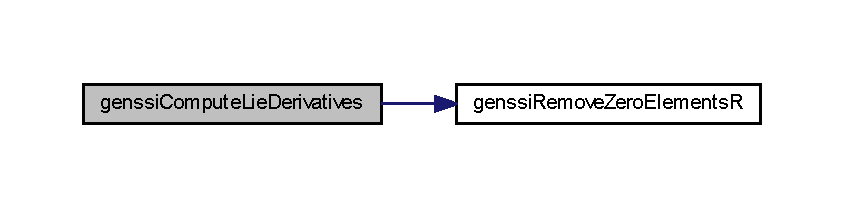
\includegraphics[width=350pt]{genssi_compute_lie_derivatives_8m_acf0ab1dc4da7184e89d949c4c30985f2_cgraph}
\end{center}
\end{figure}




Here is the caller graph for this function\+:\nopagebreak
\begin{figure}[H]
\begin{center}
\leavevmode
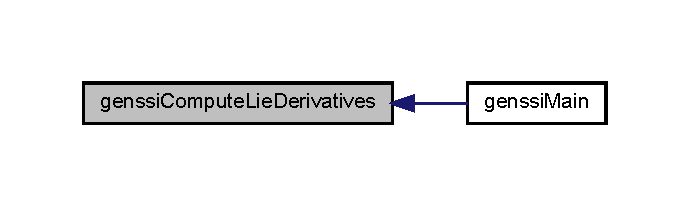
\includegraphics[width=325pt]{genssi_compute_lie_derivatives_8m_acf0ab1dc4da7184e89d949c4c30985f2_icgraph}
\end{center}
\end{figure}



\hypertarget{genssi_compute_reduced_tableau_8m}{}\subsection{Auxiliary/genssi\+Compute\+Reduced\+Tableau.m File Reference}
\label{genssi_compute_reduced_tableau_8m}\index{Auxiliary/genssi\+Compute\+Reduced\+Tableau.\+m@{Auxiliary/genssi\+Compute\+Reduced\+Tableau.\+m}}


genssi\+Compute\+Reduced\+Tableau computes reduced tableaus of the jacobian by eliminating rows and columns where solutions to relationships can found or excluded.  


\subsubsection*{Functions}
\begin{DoxyCompactItemize}
\item 
mlhs\+Subst$<$ mlhs\+Inner\+Subst$<$ matlabtypesubstitute $>$,mlhs\+Inner\+Subst$<$ matlabtypesubstitute $>$,mlhs\+Inner\+Subst$<$ matlabtypesubstitute $>$,mlhs\+Inner\+Subst$<$ matlabtypesubstitute $>$,mlhs\+Inner\+Subst$<$ matlabtypesubstitute $>$ $>$ \hyperlink{genssi_compute_reduced_tableau_8m_ac656317846d242aa597f059c664ecac1}{genssi\+Compute\+Reduced\+Tableau} (matlabtypesubstitute model, matlabtypesubstitute results, matlabtypesubstitute Vector\+Lie\+Derivatives, matlabtypesubstitute Jac\+Param, matlabtypesubstitute options)
\begin{DoxyCompactList}\small\item\em genssi\+Compute\+Reduced\+Tableau computes reduced tableaus of the jacobian by eliminating rows and columns where solutions to relationships can found or excluded. \end{DoxyCompactList}\end{DoxyCompactItemize}


\subsubsection{Function Documentation}
\mbox{\Hypertarget{genssi_compute_reduced_tableau_8m_ac656317846d242aa597f059c664ecac1}\label{genssi_compute_reduced_tableau_8m_ac656317846d242aa597f059c664ecac1}} 
\index{genssi\+Compute\+Reduced\+Tableau.\+m@{genssi\+Compute\+Reduced\+Tableau.\+m}!genssi\+Compute\+Reduced\+Tableau@{genssi\+Compute\+Reduced\+Tableau}}
\index{genssi\+Compute\+Reduced\+Tableau@{genssi\+Compute\+Reduced\+Tableau}!genssi\+Compute\+Reduced\+Tableau.\+m@{genssi\+Compute\+Reduced\+Tableau.\+m}}
\paragraph{\texorpdfstring{genssi\+Compute\+Reduced\+Tableau()}{genssiComputeReducedTableau()}}
{\footnotesize\ttfamily mlhs\+Subst$<$ mlhs\+Inner\+Subst$<$ matlabtypesubstitute $>$,mlhs\+Inner\+Subst$<$ matlabtypesubstitute $>$,mlhs\+Inner\+Subst$<$ matlabtypesubstitute $>$,mlhs\+Inner\+Subst$<$ matlabtypesubstitute $>$,mlhs\+Inner\+Subst$<$ matlabtypesubstitute $>$ $>$ genssi\+Compute\+Reduced\+Tableau (\begin{DoxyParamCaption}\item[{matlabtypesubstitute}]{model,  }\item[{matlabtypesubstitute}]{results,  }\item[{matlabtypesubstitute}]{Vector\+Lie\+Derivatives,  }\item[{matlabtypesubstitute}]{Jac\+Param,  }\item[{matlabtypesubstitute}]{options }\end{DoxyParamCaption})}


\begin{DoxyParams}{Parameters}
{\em model} & model definition (struct) \\
\hline
{\em results} & results of compute tableau (symbolic matrix) \\
\hline
{\em Vector\+Lie\+Derivatives} & vector of Lie derivatives (symbolic array) \\
\hline
{\em Jac\+Param} & jacobian with respect to parameters (symbolic matrix) \\
\hline
{\em options} & options (struct)\\
\hline
\end{DoxyParams}

\begin{DoxyRetVals}{Return values}
{\em options} & options (struct) \\
\hline
{\em results} & results of compute tableau (symbolic matrix) \\
\hline
{\em R\+Jac\+Param01} & reduced tableau (binary matrix) \\
\hline
{\em E\+CC} & equations (symbolic matrix) \\
\hline
{\em r\+Param} & reduced list of parameters (symbolic array) \\
\hline
\end{DoxyRetVals}


Definition at line 17 of file genssi\+Compute\+Reduced\+Tableau.\+m.

Here is the call graph for this function\+:\nopagebreak
\begin{figure}[H]
\begin{center}
\leavevmode
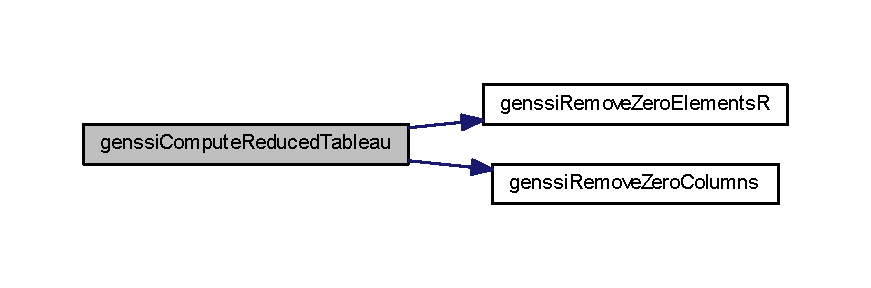
\includegraphics[width=350pt]{genssi_compute_reduced_tableau_8m_ac656317846d242aa597f059c664ecac1_cgraph}
\end{center}
\end{figure}
Here is the caller graph for this function\+:\nopagebreak
\begin{figure}[H]
\begin{center}
\leavevmode
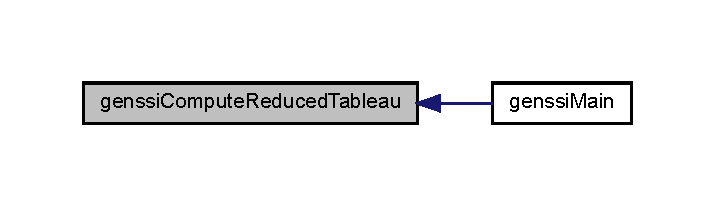
\includegraphics[width=343pt]{genssi_compute_reduced_tableau_8m_ac656317846d242aa597f059c664ecac1_icgraph}
\end{center}
\end{figure}

\hypertarget{genssi_compute_tableau_8m}{}\subsection{genssi\+Compute\+Tableau.\+m File Reference}
\label{genssi_compute_tableau_8m}\index{genssi\+Compute\+Tableau.\+m@{genssi\+Compute\+Tableau.\+m}}


genssi\+Compute\+Tableau computes the tableau based on the jacobian of the Lie derivatives.  


\subsubsection*{Functions}
\begin{DoxyCompactItemize}
\item 
mlhs\+Subst$<$ mlhs\+Inner\+Subst$<$ matlabtypesubstitute $>$,mlhs\+Inner\+Subst$<$ matlabtypesubstitute $>$,mlhs\+Inner\+Subst$<$ matlabtypesubstitute $>$ $>$ \hyperlink{genssi_compute_tableau_8m_ac36d23be66de6a962b909131c3b8f5b0}{genssi\+Compute\+Tableau} (matlabtypesubstitute model, matlabtypesubstitute Vector\+Lie\+Derivatives, matlabtypesubstitute options)
\begin{DoxyCompactList}\small\item\em genssi\+Compute\+Tableau computes the tableau based on the jacobian of the Lie derivatives. \end{DoxyCompactList}\end{DoxyCompactItemize}


\subsubsection{Function Documentation}
\index{genssi\+Compute\+Tableau.\+m@{genssi\+Compute\+Tableau.\+m}!genssi\+Compute\+Tableau@{genssi\+Compute\+Tableau}}
\index{genssi\+Compute\+Tableau@{genssi\+Compute\+Tableau}!genssi\+Compute\+Tableau.\+m@{genssi\+Compute\+Tableau.\+m}}
\paragraph[{\texorpdfstring{genssi\+Compute\+Tableau(matlabtypesubstitute model, matlabtypesubstitute Vector\+Lie\+Derivatives, matlabtypesubstitute options)}{genssiComputeTableau(matlabtypesubstitute model, matlabtypesubstitute VectorLieDerivatives, matlabtypesubstitute options)}}]{\setlength{\rightskip}{0pt plus 5cm}mlhs\+Subst$<$ mlhs\+Inner\+Subst$<$ matlabtypesubstitute $>$,mlhs\+Inner\+Subst$<$ matlabtypesubstitute $>$,mlhs\+Inner\+Subst$<$ matlabtypesubstitute $>$ $>$ genssi\+Compute\+Tableau (
\begin{DoxyParamCaption}
\item[{matlabtypesubstitute}]{model, }
\item[{matlabtypesubstitute}]{Vector\+Lie\+Derivatives, }
\item[{matlabtypesubstitute}]{options}
\end{DoxyParamCaption}
)}\hypertarget{genssi_compute_tableau_8m_ac36d23be66de6a962b909131c3b8f5b0}{}\label{genssi_compute_tableau_8m_ac36d23be66de6a962b909131c3b8f5b0}

\begin{DoxyParams}{Parameters}
{\em model} & model definition (struct) \\
\hline
{\em Vector\+Lie\+Derivatives} & vector of Lie derivatives (symbolic array) \\
\hline
{\em options} & options (struct)\\
\hline
\end{DoxyParams}

\begin{DoxyRetVals}{Return values}
{\em options} & options (struct) \\
\hline
{\em results} & results of calculations (struct) \\
\hline
{\em Jac\+Param} & jacobian of the Lie derivatives with respect to the parameters (symbolic matrix) \\
\hline
\end{DoxyRetVals}


Definition at line 17 of file genssi\+Compute\+Tableau.\+m.



Here is the call graph for this function\+:
\nopagebreak
\begin{figure}[H]
\begin{center}
\leavevmode
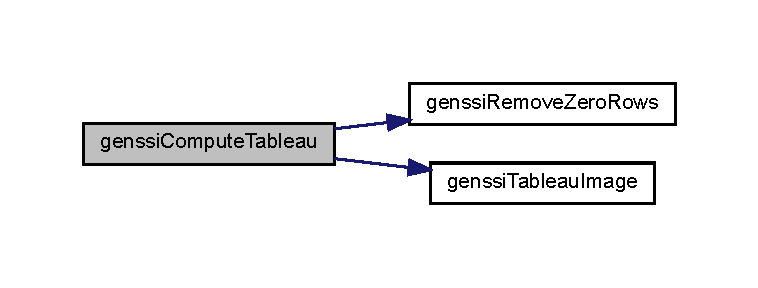
\includegraphics[width=350pt]{genssi_compute_tableau_8m_ac36d23be66de6a962b909131c3b8f5b0_cgraph}
\end{center}
\end{figure}




Here is the caller graph for this function\+:\nopagebreak
\begin{figure}[H]
\begin{center}
\leavevmode
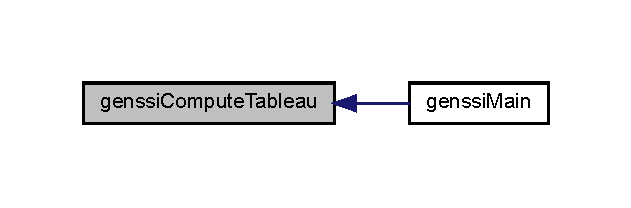
\includegraphics[width=300pt]{genssi_compute_tableau_8m_ac36d23be66de6a962b909131c3b8f5b0_icgraph}
\end{center}
\end{figure}



\hypertarget{genssi_from_amici_8m}{}\subsection{genssi\+From\+Amici.\+m File Reference}
\label{genssi_from_amici_8m}\index{genssi\+From\+Amici.\+m@{genssi\+From\+Amici.\+m}}


genssi\+From\+Amici converts an A\+M\+I\+CI model in the examples/\+A\+M\+I\+CI directory to a Gen\+S\+SI model and puts the results into the examples directory.  


\subsubsection*{Functions}
\begin{DoxyCompactItemize}
\item 
mlhs\+Inner\+Subst$<$ matlabtypesubstitute $>$ \hyperlink{genssi_from_amici_8m_aa177acfd2eae54685d2487430b93091e}{genssi\+From\+Amici} (matlabtypesubstitute model\+Name\+In, matlabtypesubstitute model\+Name\+Out)
\begin{DoxyCompactList}\small\item\em genssi\+From\+Amici converts an A\+M\+I\+CI model in the examples/\+A\+M\+I\+CI directory to a Gen\+S\+SI model and puts the results into the examples directory. \end{DoxyCompactList}\end{DoxyCompactItemize}


\subsubsection{Function Documentation}
\mbox{\Hypertarget{genssi_from_amici_8m_aa177acfd2eae54685d2487430b93091e}\label{genssi_from_amici_8m_aa177acfd2eae54685d2487430b93091e}} 
\index{genssi\+From\+Amici.\+m@{genssi\+From\+Amici.\+m}!genssi\+From\+Amici@{genssi\+From\+Amici}}
\index{genssi\+From\+Amici@{genssi\+From\+Amici}!genssi\+From\+Amici.\+m@{genssi\+From\+Amici.\+m}}
\paragraph{\texorpdfstring{genssi\+From\+Amici()}{genssiFromAmici()}}
{\footnotesize\ttfamily mlhs\+Inner\+Subst$<$ matlabtypesubstitute $>$ genssi\+From\+Amici (\begin{DoxyParamCaption}\item[{matlabtypesubstitute}]{model\+Name\+In,  }\item[{matlabtypesubstitute}]{model\+Name\+Out }\end{DoxyParamCaption})}


\begin{DoxyParams}{Parameters}
{\em model\+Name\+In} & name of the A\+M\+I\+CI model (string) \\
\hline
{\em model\+Name\+Out} & name of the Gen\+S\+SI model (string)\\
\hline
\end{DoxyParams}

\begin{DoxyRetVals}{Return values}
{\em model\+Name\+Out} & void \\
\hline
\end{DoxyRetVals}


Definition at line 17 of file genssi\+From\+Amici.\+m.

Here is the call graph for this function\+:\nopagebreak
\begin{figure}[H]
\begin{center}
\leavevmode
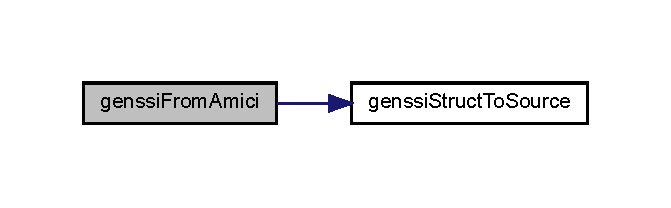
\includegraphics[width=322pt]{genssi_from_amici_8m_aa177acfd2eae54685d2487430b93091e_cgraph}
\end{center}
\end{figure}
Here is the caller graph for this function\+:\nopagebreak
\begin{figure}[H]
\begin{center}
\leavevmode
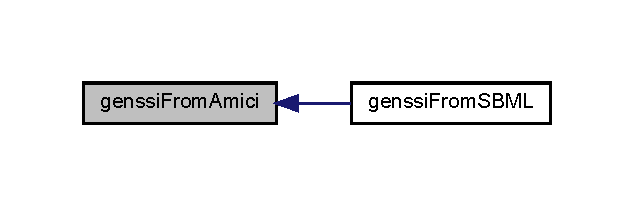
\includegraphics[width=304pt]{genssi_from_amici_8m_aa177acfd2eae54685d2487430b93091e_icgraph}
\end{center}
\end{figure}

\hypertarget{genssi_jacobian2_d_8m}{}\subsection{genssi\+Jacobian2\+D.\+m File Reference}
\label{genssi_jacobian2_d_8m}\index{genssi\+Jacobian2\+D.\+m@{genssi\+Jacobian2\+D.\+m}}


jacobian of 2D matrix, calculated as in M\+A\+P\+LE  


\subsubsection*{Functions}
\begin{DoxyCompactItemize}
\item 
mlhs\+Inner\+Subst$<$ matlabtypesubstitute $>$ \hyperlink{genssi_jacobian2_d_8m_ad10bfd468af34a31cb34aef66556c43d}{Gen\+Ssi\+Jacobian2D} (matlabtypesubstitute f, matlabtypesubstitute v)\hypertarget{genssi_jacobian2_d_8m_ad10bfd468af34a31cb34aef66556c43d}{}\label{genssi_jacobian2_d_8m_ad10bfd468af34a31cb34aef66556c43d}

\begin{DoxyCompactList}\small\item\em jacobian of 2D matrix, calculated as in M\+A\+P\+LE \end{DoxyCompactList}\end{DoxyCompactItemize}

\hypertarget{genssi_main_8m}{}\subsection{genssi\+Main.\+m File Reference}
\label{genssi_main_8m}\index{genssi\+Main.\+m@{genssi\+Main.\+m}}


genssi\+Main is the main function of Gen\+S\+SI. It reads a model and calls all other functions necessary for analyzing the model.  


\subsubsection*{Functions}
\begin{DoxyCompactItemize}
\item 
mlhs\+Inner\+Subst$<$ matlabtypesubstitute $>$ \hyperlink{genssi_main_8m_aac78e2620e69e2ecf610a2526a32c7fb}{genssi\+Main} (matlabtypesubstitute varargin)
\begin{DoxyCompactList}\small\item\em genssi\+Main is the main function of Gen\+S\+SI. It reads a model and calls all other functions necessary for analyzing the model. \end{DoxyCompactList}\end{DoxyCompactItemize}


\subsubsection{Function Documentation}
\index{genssi\+Main.\+m@{genssi\+Main.\+m}!genssi\+Main@{genssi\+Main}}
\index{genssi\+Main@{genssi\+Main}!genssi\+Main.\+m@{genssi\+Main.\+m}}
\paragraph[{\texorpdfstring{genssi\+Main(matlabtypesubstitute varargin)}{genssiMain(matlabtypesubstitute varargin)}}]{\setlength{\rightskip}{0pt plus 5cm}mlhs\+Inner\+Subst$<$ matlabtypesubstitute $>$ genssi\+Main (
\begin{DoxyParamCaption}
\item[{matlabtypesubstitute}]{varargin}
\end{DoxyParamCaption}
)}\hypertarget{genssi_main_8m_aac78e2620e69e2ecf610a2526a32c7fb}{}\label{genssi_main_8m_aac78e2620e69e2ecf610a2526a32c7fb}

\begin{DoxyParams}{Parameters}
{\em varargin} & generic input arguments 
\begin{DoxyCode}
1 genssiMain ( modelName, fileFormat, model, mat ) 
\end{DoxyCode}
 {\itshape Required Parameters for varargin\+:}
\begin{DoxyItemize}
\item  model\+Name the name of the model to be analyzed (a string)
\item  file\+Format the format of the model file
\item  model (default) if the model is a function file (e.\+g. Goodwinn.\+m)
\item  mat if the model is a Matlab file (e.\+g. Goodwin.\+mat)
\end{DoxyItemize}\\
\hline
\end{DoxyParams}

\begin{DoxyRetVals}{Return values}
{\em varargout} & generic output arguments \\
\hline
{\em options} & struct containing options \\
\hline
\end{DoxyRetVals}


Definition at line 17 of file genssi\+Main.\+m.



Here is the call graph for this function\+:
\nopagebreak
\begin{figure}[H]
\begin{center}
\leavevmode
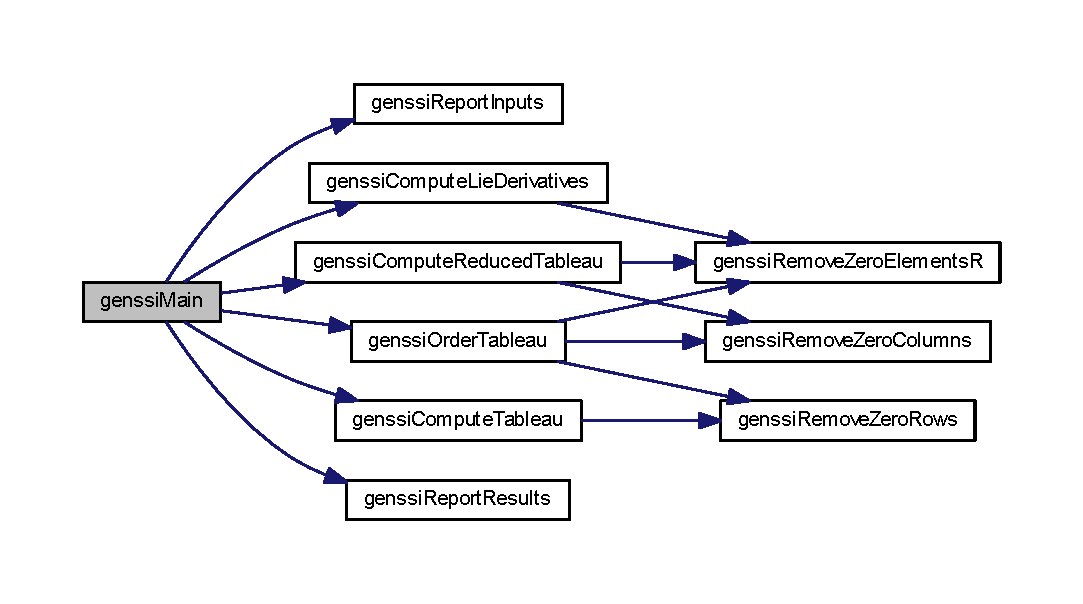
\includegraphics[width=350pt]{genssi_main_8m_aac78e2620e69e2ecf610a2526a32c7fb_cgraph}
\end{center}
\end{figure}



\hypertarget{genssi_order_tableau_8m}{}\subsection{Auxiliary/genssi\+Order\+Tableau.m File Reference}
\label{genssi_order_tableau_8m}\index{Auxiliary/genssi\+Order\+Tableau.\+m@{Auxiliary/genssi\+Order\+Tableau.\+m}}


genssi\+Order\+Tableau orders tableaus, searches for new opportunities to eliminate rows or columns be solving equations, and creates new (reduced) tableaus.  


\subsubsection*{Functions}
\begin{DoxyCompactItemize}
\item 
mlhs\+Subst$<$ mlhs\+Inner\+Subst$<$ matlabtypesubstitute $>$,mlhs\+Inner\+Subst$<$ matlabtypesubstitute $>$ $>$ \hyperlink{genssi_order_tableau_8m_aa6a1ccc8edfe7bfb0dc157b05f76bc43}{genssi\+Order\+Tableau} (matlabtypesubstitute model, matlabtypesubstitute results, matlabtypesubstitute R\+Jac\+Param01, matlabtypesubstitute E\+CC, matlabtypesubstitute r\+Param, matlabtypesubstitute options)
\begin{DoxyCompactList}\small\item\em genssi\+Order\+Tableau orders tableaus, searches for new opportunities to eliminate rows or columns be solving equations, and creates new (reduced) tableaus. \end{DoxyCompactList}\item 
\mbox{\Hypertarget{genssi_order_tableau_8m_af6cac42e06df507ddf85db9f8500ba9c}\label{genssi_order_tableau_8m_af6cac42e06df507ddf85db9f8500ba9c}} 
mlhs\+Subst$<$ mlhs\+Inner\+Subst$<$ matlabtypesubstitute $>$,mlhs\+Inner\+Subst$<$ matlabtypesubstitute $>$,mlhs\+Inner\+Subst$<$ matlabtypesubstitute $>$,mlhs\+Inner\+Subst$<$ matlabtypesubstitute $>$,mlhs\+Inner\+Subst$<$ matlabtypesubstitute $>$,mlhs\+Inner\+Subst$<$ matlabtypesubstitute $>$,mlhs\+Inner\+Subst$<$ matlabtypesubstitute $>$ $>$ \hyperlink{genssi_order_tableau_8m_af6cac42e06df507ddf85db9f8500ba9c}{mtoc\+\_\+subst\+\_\+genssi\+Order\+Tableau\+\_\+m\+\_\+tsbus\+\_\+cotm\+\_\+display\+Relevant\+Parameters} (matlabtypesubstitute Param, matlabtypesubstitute Param\+\_\+local, matlabtypesubstitute global\+\_\+ident\+\_\+par, matlabtypesubstitute Mat\+\_\+index, matlabtypesubstitute R\+Jacparam\+\_\+new, matlabtypesubstitute R\+Jac\+Param01\+\_\+nonzero\+\_\+rows, matlabtypesubstitute sum\+\_\+\+R\+Jac\+Param01\+\_\+nonzero\+\_\+rows\+\_\+t, matlabtypesubstitute E\+CC, matlabtypesubstitute E\+C\+C\+\_\+new, matlabtypesubstitute options)
\begin{DoxyCompactList}\small\item\em display\+Relevant\+Parameters displays relevant parameters \end{DoxyCompactList}\item 
\mbox{\Hypertarget{genssi_order_tableau_8m_aed9f430886899d1a0960b20d72813de6}\label{genssi_order_tableau_8m_aed9f430886899d1a0960b20d72813de6}} 
mlhs\+Subst$<$ mlhs\+Inner\+Subst$<$ matlabtypesubstitute $>$,mlhs\+Inner\+Subst$<$ matlabtypesubstitute $>$,mlhs\+Inner\+Subst$<$ matlabtypesubstitute $>$,mlhs\+Inner\+Subst$<$ matlabtypesubstitute $>$,mlhs\+Inner\+Subst$<$ matlabtypesubstitute $>$,mlhs\+Inner\+Subst$<$ matlabtypesubstitute $>$ $>$ \hyperlink{genssi_order_tableau_8m_aed9f430886899d1a0960b20d72813de6}{mtoc\+\_\+subst\+\_\+genssi\+Order\+Tableau\+\_\+m\+\_\+tsbus\+\_\+cotm\+\_\+display\+Reduced\+Tableau} (matlabtypesubstitute E\+C\+C\+\_\+remaining, matlabtypesubstitute Param\+\_\+local, matlabtypesubstitute Param\+\_\+display, matlabtypesubstitute global\+\_\+ident\+\_\+par, matlabtypesubstitute display\+\_\+tableau\+\_\+\+R\+Jacparam\+\_\+new, matlabtypesubstitute number\+\_\+fig, matlabtypesubstitute options)
\begin{DoxyCompactList}\small\item\em display\+Reduced\+Tableau displays reduced tableaus \end{DoxyCompactList}\item 
\mbox{\Hypertarget{genssi_order_tableau_8m_a9c39dab9b385b1d56975e07dabc3eff5}\label{genssi_order_tableau_8m_a9c39dab9b385b1d56975e07dabc3eff5}} 
mlhs\+Subst$<$ mlhs\+Inner\+Subst$<$ matlabtypesubstitute $>$,mlhs\+Inner\+Subst$<$ matlabtypesubstitute $>$ $>$ \hyperlink{genssi_order_tableau_8m_a9c39dab9b385b1d56975e07dabc3eff5}{mtoc\+\_\+subst\+\_\+genssi\+Order\+Tableau\+\_\+m\+\_\+tsbus\+\_\+cotm\+\_\+display\+Remaining\+Parameters} (matlabtypesubstitute E\+C\+C\+\_\+remaining, matlabtypesubstitute Param\+\_\+local, matlabtypesubstitute Param\+\_\+remaining, matlabtypesubstitute global\+\_\+ident\+\_\+par, matlabtypesubstitute display\+\_\+tableau\+\_\+\+R\+Jacparam\+\_\+new, matlabtypesubstitute row\+\_\+index\+\_\+1, matlabtypesubstitute tableau\+\_\+for\+\_\+second\+\_\+reduced\+\_\+tableau, matlabtypesubstitute parameters\+\_\+for\+\_\+second\+\_\+reduced\+\_\+tableau, matlabtypesubstitute number\+\_\+fig, matlabtypesubstitute options)
\begin{DoxyCompactList}\small\item\em display\+Reduced\+Tableau displays the remaining parameters \end{DoxyCompactList}\item 
\mbox{\Hypertarget{genssi_order_tableau_8m_a74162776b07ac9bc7800f54f65f723e7}\label{genssi_order_tableau_8m_a74162776b07ac9bc7800f54f65f723e7}} 
mlhs\+Subst$<$ mlhs\+Inner\+Subst$<$ matlabtypesubstitute $>$,mlhs\+Inner\+Subst$<$ matlabtypesubstitute $>$ $>$ \hyperlink{genssi_order_tableau_8m_a74162776b07ac9bc7800f54f65f723e7}{mtoc\+\_\+subst\+\_\+genssi\+Order\+Tableau\+\_\+m\+\_\+tsbus\+\_\+cotm\+\_\+solve\+Rem\+Par} (matlabtypesubstitute E\+CC, matlabtypesubstitute Param, matlabtypesubstitute Param\+\_\+local, matlabtypesubstitute global\+\_\+ident\+\_\+par)
\begin{DoxyCompactList}\small\item\em solve\+Rem\+Par solves the remaining parameters \end{DoxyCompactList}\item 
\mbox{\Hypertarget{genssi_order_tableau_8m_a138fca3f232c92c207f047feff4453a6}\label{genssi_order_tableau_8m_a138fca3f232c92c207f047feff4453a6}} 
mlhs\+Subst$<$ mlhs\+Inner\+Subst$<$ matlabtypesubstitute $>$,mlhs\+Inner\+Subst$<$ matlabtypesubstitute $>$ $>$ \hyperlink{genssi_order_tableau_8m_a138fca3f232c92c207f047feff4453a6}{mtoc\+\_\+subst\+\_\+genssi\+Order\+Tableau\+\_\+m\+\_\+tsbus\+\_\+cotm\+\_\+get\+Index\+Of\+Duplicate\+Params} (matlabtypesubstitute E\+CC, matlabtypesubstitute R\+Jac\+Param01\+\_\+nonzero\+\_\+rows)
\begin{DoxyCompactList}\small\item\em get\+Index\+Of\+Duplicate\+Params gets index of duplicate parameters \end{DoxyCompactList}\end{DoxyCompactItemize}


\subsubsection{Function Documentation}
\mbox{\Hypertarget{genssi_order_tableau_8m_aa6a1ccc8edfe7bfb0dc157b05f76bc43}\label{genssi_order_tableau_8m_aa6a1ccc8edfe7bfb0dc157b05f76bc43}} 
\index{genssi\+Order\+Tableau.\+m@{genssi\+Order\+Tableau.\+m}!genssi\+Order\+Tableau@{genssi\+Order\+Tableau}}
\index{genssi\+Order\+Tableau@{genssi\+Order\+Tableau}!genssi\+Order\+Tableau.\+m@{genssi\+Order\+Tableau.\+m}}
\paragraph{\texorpdfstring{genssi\+Order\+Tableau()}{genssiOrderTableau()}}
{\footnotesize\ttfamily mlhs\+Subst$<$ mlhs\+Inner\+Subst$<$ matlabtypesubstitute $>$,mlhs\+Inner\+Subst$<$ matlabtypesubstitute $>$ $>$ genssi\+Order\+Tableau (\begin{DoxyParamCaption}\item[{matlabtypesubstitute}]{model,  }\item[{matlabtypesubstitute}]{results,  }\item[{matlabtypesubstitute}]{R\+Jac\+Param01,  }\item[{matlabtypesubstitute}]{E\+CC,  }\item[{matlabtypesubstitute}]{r\+Param,  }\item[{matlabtypesubstitute}]{options }\end{DoxyParamCaption})}


\begin{DoxyParams}{Parameters}
{\em model} & model definition (struct) \\
\hline
{\em results} & results of previous steps (struct) \\
\hline
{\em R\+Jac\+Param01} & reduced tableau, i.\+e. binary form of jacobian of the Lie derivatives with respect to the parameters (binary matrix) \\
\hline
{\em E\+CC} & equations (symbolic array) \\
\hline
{\em r\+Param} & reduced list of parameters (symbolic array) \\
\hline
{\em options} & options (struct)\\
\hline
\end{DoxyParams}

\begin{DoxyRetVals}{Return values}
{\em options} & options (struct) \\
\hline
{\em results} & results of previous steps (struct) \\
\hline
\end{DoxyRetVals}


Definition at line 17 of file genssi\+Order\+Tableau.\+m.

Here is the call graph for this function\+:\nopagebreak
\begin{figure}[H]
\begin{center}
\leavevmode
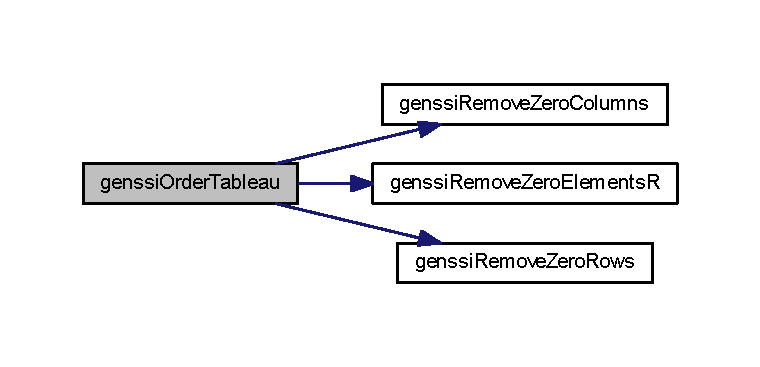
\includegraphics[width=350pt]{genssi_order_tableau_8m_aa6a1ccc8edfe7bfb0dc157b05f76bc43_cgraph}
\end{center}
\end{figure}
Here is the caller graph for this function\+:\nopagebreak
\begin{figure}[H]
\begin{center}
\leavevmode
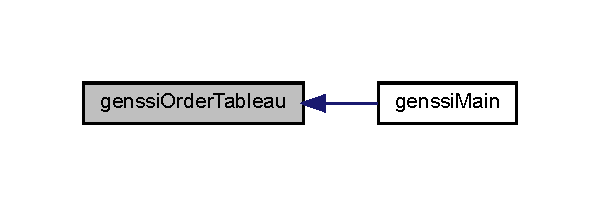
\includegraphics[width=288pt]{genssi_order_tableau_8m_aa6a1ccc8edfe7bfb0dc157b05f76bc43_icgraph}
\end{center}
\end{figure}

\hypertarget{genssi_remove_zero_columns_8m}{}\subsection{Auxiliary/genssi\+Remove\+Zero\+Columns.m File Reference}
\label{genssi_remove_zero_columns_8m}\index{Auxiliary/genssi\+Remove\+Zero\+Columns.\+m@{Auxiliary/genssi\+Remove\+Zero\+Columns.\+m}}


genssi\+Remove\+Zero\+Columns removes zero columns from a matrix  


\subsubsection*{Functions}
\begin{DoxyCompactItemize}
\item 
mlhs\+Subst$<$ mlhs\+Inner\+Subst$<$ matlabtypesubstitute $>$,mlhs\+Inner\+Subst$<$ matlabtypesubstitute $>$,mlhs\+Inner\+Subst$<$ matlabtypesubstitute $>$ $>$ \hyperlink{genssi_remove_zero_columns_8m_af18483f4677ea487d40a6a08b6d61a6e}{genssi\+Remove\+Zero\+Columns} (matlabtypesubstitute matrix\+In)
\begin{DoxyCompactList}\small\item\em genssi\+Remove\+Zero\+Columns removes zero columns from a matrix \end{DoxyCompactList}\end{DoxyCompactItemize}


\subsubsection{Function Documentation}
\mbox{\Hypertarget{genssi_remove_zero_columns_8m_af18483f4677ea487d40a6a08b6d61a6e}\label{genssi_remove_zero_columns_8m_af18483f4677ea487d40a6a08b6d61a6e}} 
\index{genssi\+Remove\+Zero\+Columns.\+m@{genssi\+Remove\+Zero\+Columns.\+m}!genssi\+Remove\+Zero\+Columns@{genssi\+Remove\+Zero\+Columns}}
\index{genssi\+Remove\+Zero\+Columns@{genssi\+Remove\+Zero\+Columns}!genssi\+Remove\+Zero\+Columns.\+m@{genssi\+Remove\+Zero\+Columns.\+m}}
\paragraph{\texorpdfstring{genssi\+Remove\+Zero\+Columns()}{genssiRemoveZeroColumns()}}
{\footnotesize\ttfamily mlhs\+Subst$<$ mlhs\+Inner\+Subst$<$ matlabtypesubstitute $>$,mlhs\+Inner\+Subst$<$ matlabtypesubstitute $>$,mlhs\+Inner\+Subst$<$ matlabtypesubstitute $>$ $>$ genssi\+Remove\+Zero\+Columns (\begin{DoxyParamCaption}\item[{matlabtypesubstitute}]{matrix\+In }\end{DoxyParamCaption})}


\begin{DoxyParams}{Parameters}
{\em matrix\+In} & input (matrix)\\
\hline
\end{DoxyParams}

\begin{DoxyRetVals}{Return values}
{\em matrix\+Out} & output (matrix) \\
\hline
{\em keep\+Boolean} & boolean vector of indices kept (array) \\
\hline
{\em keep\+Index} & vector of indices keept (array) \\
\hline
\end{DoxyRetVals}


Definition at line 17 of file genssi\+Remove\+Zero\+Columns.\+m.

Here is the caller graph for this function\+:\nopagebreak
\begin{figure}[H]
\begin{center}
\leavevmode
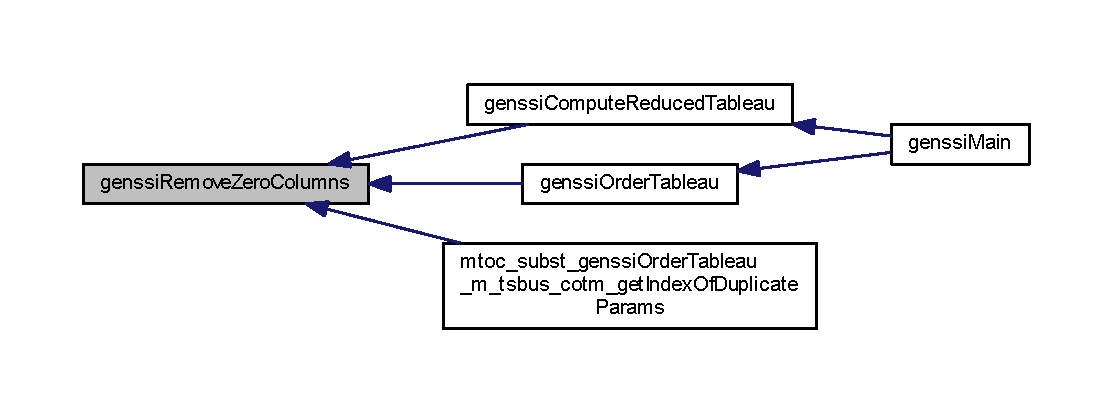
\includegraphics[width=350pt]{genssi_remove_zero_columns_8m_af18483f4677ea487d40a6a08b6d61a6e_icgraph}
\end{center}
\end{figure}

\hypertarget{genssi_remove_zero_elements_c_8m}{}\subsection{genssi\+Remove\+Zero\+Elements\+C.\+m File Reference}
\label{genssi_remove_zero_elements_c_8m}\index{genssi\+Remove\+Zero\+Elements\+C.\+m@{genssi\+Remove\+Zero\+Elements\+C.\+m}}


genssi\+Remove\+Zero\+Elements removes zero columns from a row vecor  


\subsubsection*{Functions}
\begin{DoxyCompactItemize}
\item 
mlhs\+Subst$<$ mlhs\+Inner\+Subst$<$ matlabtypesubstitute $>$,mlhs\+Inner\+Subst$<$ matlabtypesubstitute $>$,mlhs\+Inner\+Subst$<$ matlabtypesubstitute $>$ $>$ \hyperlink{genssi_remove_zero_elements_c_8m_a8c28e35503c10ad2d08254f923d3ba38}{genssi\+Remove\+Zero\+ElementsC} (matlabtypesubstitute vector\+In)
\begin{DoxyCompactList}\small\item\em genssi\+Remove\+Zero\+Elements removes zero columns from a row vecor \end{DoxyCompactList}\end{DoxyCompactItemize}


\subsubsection{Function Documentation}
\index{genssi\+Remove\+Zero\+Elements\+C.\+m@{genssi\+Remove\+Zero\+Elements\+C.\+m}!genssi\+Remove\+Zero\+ElementsC@{genssi\+Remove\+Zero\+ElementsC}}
\index{genssi\+Remove\+Zero\+ElementsC@{genssi\+Remove\+Zero\+ElementsC}!genssi\+Remove\+Zero\+Elements\+C.\+m@{genssi\+Remove\+Zero\+Elements\+C.\+m}}
\paragraph[{\texorpdfstring{genssi\+Remove\+Zero\+Elements\+C(matlabtypesubstitute vector\+In)}{genssiRemoveZeroElementsC(matlabtypesubstitute vectorIn)}}]{\setlength{\rightskip}{0pt plus 5cm}mlhs\+Subst$<$ mlhs\+Inner\+Subst$<$ matlabtypesubstitute $>$,mlhs\+Inner\+Subst$<$ matlabtypesubstitute $>$,mlhs\+Inner\+Subst$<$ matlabtypesubstitute $>$ $>$ genssi\+Remove\+Zero\+ElementsC (
\begin{DoxyParamCaption}
\item[{matlabtypesubstitute}]{vector\+In}
\end{DoxyParamCaption}
)}\hypertarget{genssi_remove_zero_elements_c_8m_a8c28e35503c10ad2d08254f923d3ba38}{}\label{genssi_remove_zero_elements_c_8m_a8c28e35503c10ad2d08254f923d3ba38}

\begin{DoxyParams}{Parameters}
{\em vector\+In} & input (array)\\
\hline
\end{DoxyParams}

\begin{DoxyRetVals}{Return values}
{\em vector\+Out} & output (array) \\
\hline
{\em keep\+Boolean} & boolean vector of indices kept (array) \\
\hline
{\em keep\+Index} & vector of indices kept (array) \\
\hline
\end{DoxyRetVals}


Definition at line 17 of file genssi\+Remove\+Zero\+Elements\+C.\+m.



Here is the caller graph for this function\+:
\nopagebreak
\begin{figure}[H]
\begin{center}
\leavevmode
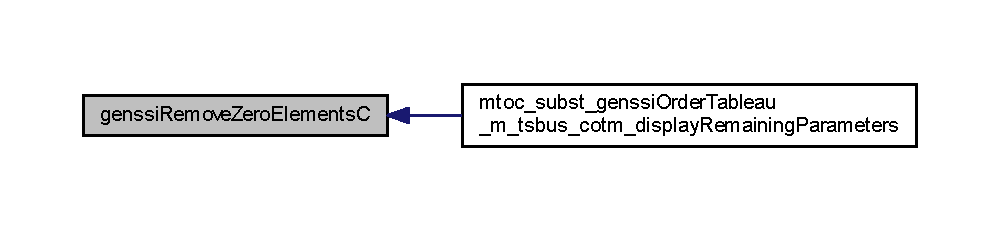
\includegraphics[width=350pt]{genssi_remove_zero_elements_c_8m_a8c28e35503c10ad2d08254f923d3ba38_icgraph}
\end{center}
\end{figure}



\hypertarget{genssi_remove_zero_elements_r_8m}{}\subsection{genssi\+Remove\+Zero\+Elements\+R.\+m File Reference}
\label{genssi_remove_zero_elements_r_8m}\index{genssi\+Remove\+Zero\+Elements\+R.\+m@{genssi\+Remove\+Zero\+Elements\+R.\+m}}


genssi\+Remove\+Zero\+Elements removes zero columns from a row vecor  


\subsubsection*{Functions}
\begin{DoxyCompactItemize}
\item 
mlhs\+Subst$<$ mlhs\+Inner\+Subst$<$ matlabtypesubstitute $>$,mlhs\+Inner\+Subst$<$ matlabtypesubstitute $>$,mlhs\+Inner\+Subst$<$ matlabtypesubstitute $>$ $>$ \hyperlink{genssi_remove_zero_elements_r_8m_ac88c8ec50dab4ae7cc829679aa5048cc}{genssi\+Remove\+Zero\+ElementsR} (matlabtypesubstitute vector\+In)
\begin{DoxyCompactList}\small\item\em genssi\+Remove\+Zero\+Elements removes zero columns from a row vecor \end{DoxyCompactList}\end{DoxyCompactItemize}


\subsubsection{Function Documentation}
\index{genssi\+Remove\+Zero\+Elements\+R.\+m@{genssi\+Remove\+Zero\+Elements\+R.\+m}!genssi\+Remove\+Zero\+ElementsR@{genssi\+Remove\+Zero\+ElementsR}}
\index{genssi\+Remove\+Zero\+ElementsR@{genssi\+Remove\+Zero\+ElementsR}!genssi\+Remove\+Zero\+Elements\+R.\+m@{genssi\+Remove\+Zero\+Elements\+R.\+m}}
\paragraph[{\texorpdfstring{genssi\+Remove\+Zero\+Elements\+R(matlabtypesubstitute vector\+In)}{genssiRemoveZeroElementsR(matlabtypesubstitute vectorIn)}}]{\setlength{\rightskip}{0pt plus 5cm}mlhs\+Subst$<$ mlhs\+Inner\+Subst$<$ matlabtypesubstitute $>$,mlhs\+Inner\+Subst$<$ matlabtypesubstitute $>$,mlhs\+Inner\+Subst$<$ matlabtypesubstitute $>$ $>$ genssi\+Remove\+Zero\+ElementsR (
\begin{DoxyParamCaption}
\item[{matlabtypesubstitute}]{vector\+In}
\end{DoxyParamCaption}
)}\hypertarget{genssi_remove_zero_elements_r_8m_ac88c8ec50dab4ae7cc829679aa5048cc}{}\label{genssi_remove_zero_elements_r_8m_ac88c8ec50dab4ae7cc829679aa5048cc}

\begin{DoxyParams}{Parameters}
{\em vector\+In} & input (array)\\
\hline
\end{DoxyParams}

\begin{DoxyRetVals}{Return values}
{\em vector\+Out} & output (array) \\
\hline
{\em keep\+Boolean} & boolean vector of indices kept (array) \\
\hline
{\em keep\+Index} & vector of indices kept (array) \\
\hline
\end{DoxyRetVals}


Definition at line 17 of file genssi\+Remove\+Zero\+Elements\+R.\+m.



Here is the caller graph for this function\+:
\nopagebreak
\begin{figure}[H]
\begin{center}
\leavevmode
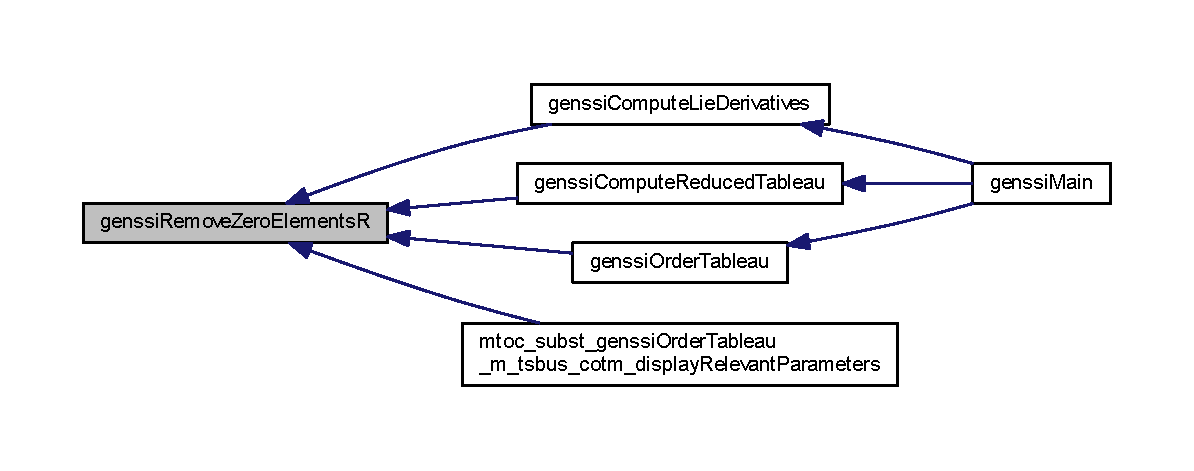
\includegraphics[width=350pt]{genssi_remove_zero_elements_r_8m_ac88c8ec50dab4ae7cc829679aa5048cc_icgraph}
\end{center}
\end{figure}



\hypertarget{genssi_remove_zero_rows_8m}{}\subsection{genssi\+Remove\+Zero\+Rows.\+m File Reference}
\label{genssi_remove_zero_rows_8m}\index{genssi\+Remove\+Zero\+Rows.\+m@{genssi\+Remove\+Zero\+Rows.\+m}}


genssi\+Remove\+Zero\+Rows removes zero rows from a matrix  


\subsubsection*{Functions}
\begin{DoxyCompactItemize}
\item 
mlhs\+Subst$<$ mlhs\+Inner\+Subst$<$ matlabtypesubstitute $>$,mlhs\+Inner\+Subst$<$ matlabtypesubstitute $>$,mlhs\+Inner\+Subst$<$ matlabtypesubstitute $>$ $>$ \hyperlink{genssi_remove_zero_rows_8m_a85d5908f175db2cb29782de20ff4e910}{genssi\+Remove\+Zero\+Rows} (matlabtypesubstitute matrix\+In)
\begin{DoxyCompactList}\small\item\em genssi\+Remove\+Zero\+Rows removes zero rows from a matrix \end{DoxyCompactList}\end{DoxyCompactItemize}


\subsubsection{Function Documentation}
\index{genssi\+Remove\+Zero\+Rows.\+m@{genssi\+Remove\+Zero\+Rows.\+m}!genssi\+Remove\+Zero\+Rows@{genssi\+Remove\+Zero\+Rows}}
\index{genssi\+Remove\+Zero\+Rows@{genssi\+Remove\+Zero\+Rows}!genssi\+Remove\+Zero\+Rows.\+m@{genssi\+Remove\+Zero\+Rows.\+m}}
\paragraph[{\texorpdfstring{genssi\+Remove\+Zero\+Rows(matlabtypesubstitute matrix\+In)}{genssiRemoveZeroRows(matlabtypesubstitute matrixIn)}}]{\setlength{\rightskip}{0pt plus 5cm}mlhs\+Subst$<$ mlhs\+Inner\+Subst$<$ matlabtypesubstitute $>$,mlhs\+Inner\+Subst$<$ matlabtypesubstitute $>$,mlhs\+Inner\+Subst$<$ matlabtypesubstitute $>$ $>$ genssi\+Remove\+Zero\+Rows (
\begin{DoxyParamCaption}
\item[{matlabtypesubstitute}]{matrix\+In}
\end{DoxyParamCaption}
)}\hypertarget{genssi_remove_zero_rows_8m_a85d5908f175db2cb29782de20ff4e910}{}\label{genssi_remove_zero_rows_8m_a85d5908f175db2cb29782de20ff4e910}

\begin{DoxyParams}{Parameters}
{\em matrix\+In} & input (matrix)\\
\hline
\end{DoxyParams}

\begin{DoxyRetVals}{Return values}
{\em matrix\+Out} & output (matrix) \\
\hline
{\em keep\+Boolean} & boolean vector of indices kept (array) \\
\hline
{\em keep\+Index} & vector of indices keept (array) \\
\hline
\end{DoxyRetVals}


Definition at line 17 of file genssi\+Remove\+Zero\+Rows.\+m.



Here is the caller graph for this function\+:
\nopagebreak
\begin{figure}[H]
\begin{center}
\leavevmode
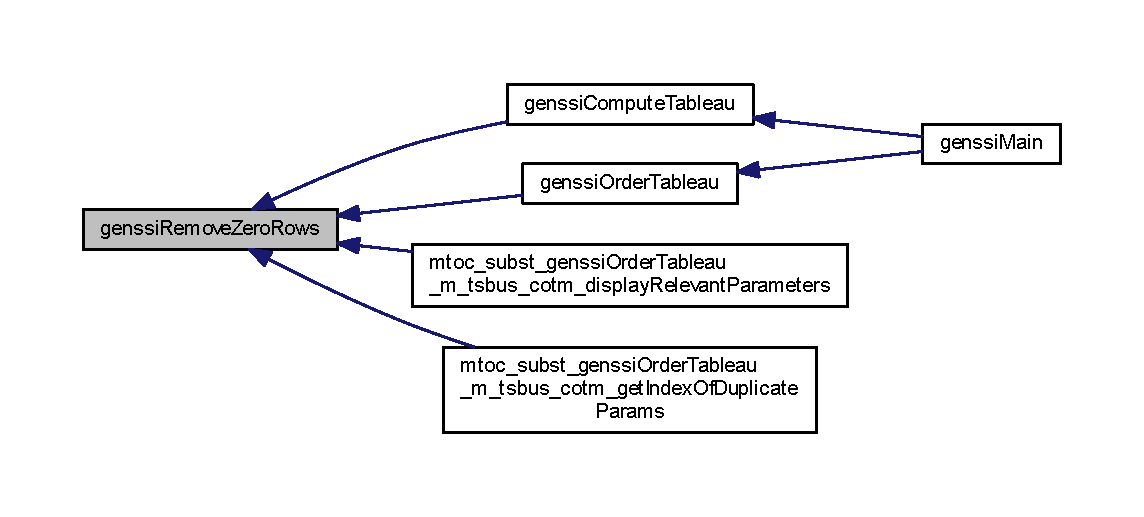
\includegraphics[width=350pt]{genssi_remove_zero_rows_8m_a85d5908f175db2cb29782de20ff4e910_icgraph}
\end{center}
\end{figure}



\hypertarget{genssi_report_inputs_8m}{}\subsection{Auxiliary/genssi\+Report\+Inputs.m File Reference}
\label{genssi_report_inputs_8m}\index{Auxiliary/genssi\+Report\+Inputs.\+m@{Auxiliary/genssi\+Report\+Inputs.\+m}}


genssi\+Report\+Inputs reports inputs, i.\+e. model definition.  


\subsubsection*{Functions}
\begin{DoxyCompactItemize}
\item 
mlhs\+Inner\+Subst$<$ matlabtypesubstitute $>$ \hyperlink{genssi_report_inputs_8m_ae09bec75fc89d3acdf984374b3f918f5}{genssi\+Report\+Inputs} (matlabtypesubstitute model, matlabtypesubstitute options)
\begin{DoxyCompactList}\small\item\em genssi\+Report\+Inputs reports inputs, i.\+e. model definition. \end{DoxyCompactList}\end{DoxyCompactItemize}


\subsubsection{Function Documentation}
\mbox{\Hypertarget{genssi_report_inputs_8m_ae09bec75fc89d3acdf984374b3f918f5}\label{genssi_report_inputs_8m_ae09bec75fc89d3acdf984374b3f918f5}} 
\index{genssi\+Report\+Inputs.\+m@{genssi\+Report\+Inputs.\+m}!genssi\+Report\+Inputs@{genssi\+Report\+Inputs}}
\index{genssi\+Report\+Inputs@{genssi\+Report\+Inputs}!genssi\+Report\+Inputs.\+m@{genssi\+Report\+Inputs.\+m}}
\paragraph{\texorpdfstring{genssi\+Report\+Inputs()}{genssiReportInputs()}}
{\footnotesize\ttfamily mlhs\+Inner\+Subst$<$ matlabtypesubstitute $>$ genssi\+Report\+Inputs (\begin{DoxyParamCaption}\item[{matlabtypesubstitute}]{model,  }\item[{matlabtypesubstitute}]{options }\end{DoxyParamCaption})}


\begin{DoxyParams}{Parameters}
{\em model} & model definition (struct) \\
\hline
{\em options} & options (struct)\\
\hline
\end{DoxyParams}

\begin{DoxyRetVals}{Return values}
{\em options} & options (struct) \\
\hline
\end{DoxyRetVals}


Definition at line 17 of file genssi\+Report\+Inputs.\+m.

Here is the caller graph for this function\+:\nopagebreak
\begin{figure}[H]
\begin{center}
\leavevmode
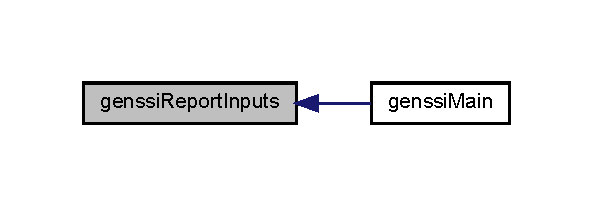
\includegraphics[width=285pt]{genssi_report_inputs_8m_ae09bec75fc89d3acdf984374b3f918f5_icgraph}
\end{center}
\end{figure}

\hypertarget{genssi_report_results_8m}{}\subsection{Auxiliary/genssi\+Report\+Results.m File Reference}
\label{genssi_report_results_8m}\index{Auxiliary/genssi\+Report\+Results.\+m@{Auxiliary/genssi\+Report\+Results.\+m}}


genssi\+Report\+Results reports the results of the analysis.  


\subsubsection*{Functions}
\begin{DoxyCompactItemize}
\item 
mlhs\+Inner\+Subst$<$ matlabtypesubstitute $>$ \hyperlink{genssi_report_results_8m_aca05cb31b560f7bf000c804036014cfc}{genssi\+Report\+Results} (matlabtypesubstitute model, matlabtypesubstitute results, matlabtypesubstitute options)
\begin{DoxyCompactList}\small\item\em genssi\+Report\+Results reports the results of the analysis. \end{DoxyCompactList}\end{DoxyCompactItemize}


\subsubsection{Function Documentation}
\mbox{\Hypertarget{genssi_report_results_8m_aca05cb31b560f7bf000c804036014cfc}\label{genssi_report_results_8m_aca05cb31b560f7bf000c804036014cfc}} 
\index{genssi\+Report\+Results.\+m@{genssi\+Report\+Results.\+m}!genssi\+Report\+Results@{genssi\+Report\+Results}}
\index{genssi\+Report\+Results@{genssi\+Report\+Results}!genssi\+Report\+Results.\+m@{genssi\+Report\+Results.\+m}}
\paragraph{\texorpdfstring{genssi\+Report\+Results()}{genssiReportResults()}}
{\footnotesize\ttfamily mlhs\+Inner\+Subst$<$ matlabtypesubstitute $>$ genssi\+Report\+Results (\begin{DoxyParamCaption}\item[{matlabtypesubstitute}]{model,  }\item[{matlabtypesubstitute}]{results,  }\item[{matlabtypesubstitute}]{options }\end{DoxyParamCaption})}


\begin{DoxyParams}{Parameters}
{\em model} & model definition (struct) \\
\hline
{\em results} & results of previous steps (struct) \\
\hline
{\em options} & options (struct)\\
\hline
\end{DoxyParams}

\begin{DoxyRetVals}{Return values}
{\em options} & options (struct) \\
\hline
\end{DoxyRetVals}


Definition at line 17 of file genssi\+Report\+Results.\+m.

Here is the caller graph for this function\+:\nopagebreak
\begin{figure}[H]
\begin{center}
\leavevmode
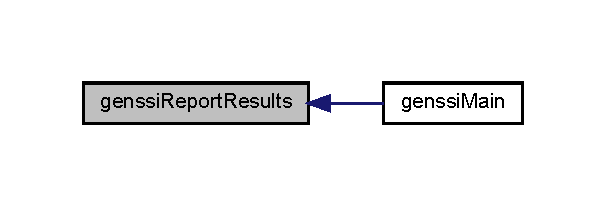
\includegraphics[width=291pt]{genssi_report_results_8m_aca05cb31b560f7bf000c804036014cfc_icgraph}
\end{center}
\end{figure}

\hypertarget{genssi_startup_8m}{}\subsection{genssi\+Startup.\+m File Reference}
\label{genssi_startup_8m}\index{genssi\+Startup.\+m@{genssi\+Startup.\+m}}


genssi\+Startup adds all paths reqquired for Gen\+S\+SI. It should be called at the beginning of a session.  


\subsubsection*{Functions}
\begin{DoxyCompactItemize}
\item 
noret\+::substitute \hyperlink{genssi_startup_8m_addcff165cb4278db5bc6df9f60bff280}{genssi\+Startup} ()\hypertarget{genssi_startup_8m_addcff165cb4278db5bc6df9f60bff280}{}\label{genssi_startup_8m_addcff165cb4278db5bc6df9f60bff280}

\begin{DoxyCompactList}\small\item\em genssi\+Startup adds all paths reqquired for Gen\+S\+SI. It should be called at the beginning of a session. \end{DoxyCompactList}\end{DoxyCompactItemize}

\hypertarget{gen_ssi_struct_to_source_8m}{}\subsection{gen\+Ssi\+Struct\+To\+Source.\+m File Reference}
\label{gen_ssi_struct_to_source_8m}\index{gen\+Ssi\+Struct\+To\+Source.\+m@{gen\+Ssi\+Struct\+To\+Source.\+m}}


gen\+Ssi\+Struct\+To\+Source converts a model definition (struct) to a source format (Matlab function file) ans saves the results in the examples directory.  


\subsubsection*{Functions}
\begin{DoxyCompactItemize}
\item 
noret\+::substitute \hyperlink{gen_ssi_struct_to_source_8m_af108169dde49ed28c9192d61c8c58846}{gen\+Ssi\+Struct\+To\+Source} (matlabtypesubstitute model)
\begin{DoxyCompactList}\small\item\em gen\+Ssi\+Struct\+To\+Source converts a model definition (struct) to a source format (Matlab function file) ans saves the results in the examples directory. \end{DoxyCompactList}\end{DoxyCompactItemize}


\subsubsection{Function Documentation}
\index{gen\+Ssi\+Struct\+To\+Source.\+m@{gen\+Ssi\+Struct\+To\+Source.\+m}!gen\+Ssi\+Struct\+To\+Source@{gen\+Ssi\+Struct\+To\+Source}}
\index{gen\+Ssi\+Struct\+To\+Source@{gen\+Ssi\+Struct\+To\+Source}!gen\+Ssi\+Struct\+To\+Source.\+m@{gen\+Ssi\+Struct\+To\+Source.\+m}}
\paragraph[{\texorpdfstring{gen\+Ssi\+Struct\+To\+Source(matlabtypesubstitute model)}{genSsiStructToSource(matlabtypesubstitute model)}}]{\setlength{\rightskip}{0pt plus 5cm}noret\+::substitute gen\+Ssi\+Struct\+To\+Source (
\begin{DoxyParamCaption}
\item[{matlabtypesubstitute}]{model}
\end{DoxyParamCaption}
)}\hypertarget{gen_ssi_struct_to_source_8m_af108169dde49ed28c9192d61c8c58846}{}\label{gen_ssi_struct_to_source_8m_af108169dde49ed28c9192d61c8c58846}

\begin{DoxyParams}{Parameters}
{\em model} & model definition (struct)\\
\hline
\end{DoxyParams}

\begin{DoxyRetVals}{Return values}
{\em model} & void \\
\hline
\end{DoxyRetVals}


Definition at line 17 of file gen\+Ssi\+Struct\+To\+Source.\+m.



Here is the caller graph for this function\+:\nopagebreak
\begin{figure}[H]
\begin{center}
\leavevmode
\includegraphics[width=334pt]{gen_ssi_struct_to_source_8m_af108169dde49ed28c9192d61c8c58846_icgraph}
\end{center}
\end{figure}



\hypertarget{genssi_to_amici_8m}{}\subsection{genssi\+To\+Amici.\+m File Reference}
\label{genssi_to_amici_8m}\index{genssi\+To\+Amici.\+m@{genssi\+To\+Amici.\+m}}


Gen\+Ssi\+To\+Amici converts a Gen\+S\+SI model to A\+M\+I\+CI model format and saves the results in the examples directory.  


\subsubsection*{Functions}
\begin{DoxyCompactItemize}
\item 
mlhs\+Inner\+Subst$<$ matlabtypesubstitute $>$ \hyperlink{genssi_to_amici_8m_a317b8cb9b241f23b1d8c0da3b37e63ee}{genssi\+To\+Amici} (matlabtypesubstitute model\+Name\+In, matlabtypesubstitute model\+Name\+Out)
\begin{DoxyCompactList}\small\item\em Gen\+Ssi\+To\+Amici converts a Gen\+S\+SI model to A\+M\+I\+CI model format and saves the results in the examples directory. \end{DoxyCompactList}\end{DoxyCompactItemize}


\subsubsection{Function Documentation}
\index{genssi\+To\+Amici.\+m@{genssi\+To\+Amici.\+m}!genssi\+To\+Amici@{genssi\+To\+Amici}}
\index{genssi\+To\+Amici@{genssi\+To\+Amici}!genssi\+To\+Amici.\+m@{genssi\+To\+Amici.\+m}}
\paragraph[{\texorpdfstring{genssi\+To\+Amici(matlabtypesubstitute model\+Name\+In, matlabtypesubstitute model\+Name\+Out)}{genssiToAmici(matlabtypesubstitute modelNameIn, matlabtypesubstitute modelNameOut)}}]{\setlength{\rightskip}{0pt plus 5cm}mlhs\+Inner\+Subst$<$ matlabtypesubstitute $>$ genssi\+To\+Amici (
\begin{DoxyParamCaption}
\item[{matlabtypesubstitute}]{model\+Name\+In, }
\item[{matlabtypesubstitute}]{model\+Name\+Out}
\end{DoxyParamCaption}
)}\hypertarget{genssi_to_amici_8m_a317b8cb9b241f23b1d8c0da3b37e63ee}{}\label{genssi_to_amici_8m_a317b8cb9b241f23b1d8c0da3b37e63ee}

\begin{DoxyParams}{Parameters}
{\em model\+Name\+In} & name of the Gen\+S\+SI model (string) \\
\hline
{\em model\+Name\+Out} & name of the A\+M\+I\+CI model (string)\\
\hline
\end{DoxyParams}

\begin{DoxyRetVals}{Return values}
{\em model\+Name\+Out} & void \\
\hline
\end{DoxyRetVals}


Definition at line 17 of file genssi\+To\+Amici.\+m.


\hypertarget{genssi_to_polynomial_8m}{}\subsection{genssi\+To\+Polynomial.\+m File Reference}
\label{genssi_to_polynomial_8m}\index{genssi\+To\+Polynomial.\+m@{genssi\+To\+Polynomial.\+m}}


genssi\+To\+Polynomial converts a Gen\+S\+SI model to polynomial form. It reads the input model, converts to polynomial form, and creates an output model as a Matlab function model\+Name\+Out.\+m and as a Matlab file modelname\+Out.\+mat, both in the Examples folder.  


\subsubsection*{Functions}
\begin{DoxyCompactItemize}
\item 
mlhs\+Inner\+Subst$<$ matlabtypesubstitute $>$ \hyperlink{genssi_to_polynomial_8m_acef0ff085917e1375d0fc2b6feed0722}{genssi\+To\+Polynomial} (matlabtypesubstitute model\+Name\+In, matlabtypesubstitute model\+Name\+Out)
\begin{DoxyCompactList}\small\item\em genssi\+To\+Polynomial converts a Gen\+S\+SI model to polynomial form. It reads the input model, converts to polynomial form, and creates an output model as a Matlab function model\+Name\+Out.\+m and as a Matlab file modelname\+Out.\+mat, both in the Examples folder. \end{DoxyCompactList}\end{DoxyCompactItemize}


\subsubsection{Function Documentation}
\mbox{\Hypertarget{genssi_to_polynomial_8m_acef0ff085917e1375d0fc2b6feed0722}\label{genssi_to_polynomial_8m_acef0ff085917e1375d0fc2b6feed0722}} 
\index{genssi\+To\+Polynomial.\+m@{genssi\+To\+Polynomial.\+m}!genssi\+To\+Polynomial@{genssi\+To\+Polynomial}}
\index{genssi\+To\+Polynomial@{genssi\+To\+Polynomial}!genssi\+To\+Polynomial.\+m@{genssi\+To\+Polynomial.\+m}}
\paragraph{\texorpdfstring{genssi\+To\+Polynomial()}{genssiToPolynomial()}}
{\footnotesize\ttfamily mlhs\+Inner\+Subst$<$ matlabtypesubstitute $>$ genssi\+To\+Polynomial (\begin{DoxyParamCaption}\item[{matlabtypesubstitute}]{model\+Name\+In,  }\item[{matlabtypesubstitute}]{model\+Name\+Out }\end{DoxyParamCaption})}


\begin{DoxyParams}{Parameters}
{\em model\+Name\+In} & the name of the input model (a string) \\
\hline
{\em model\+Name\+Out} & the name of the output model (a string)\\
\hline
\end{DoxyParams}

\begin{DoxyRetVals}{Return values}
{\em model\+Name\+Out} & void \\
\hline
\end{DoxyRetVals}


Definition at line 17 of file genssi\+To\+Polynomial.\+m.

Here is the call graph for this function\+:\nopagebreak
\begin{figure}[H]
\begin{center}
\leavevmode
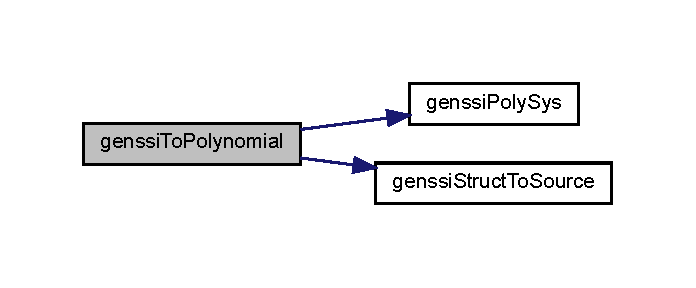
\includegraphics[width=334pt]{genssi_to_polynomial_8m_acef0ff085917e1375d0fc2b6feed0722_cgraph}
\end{center}
\end{figure}

%--- End generated contents ---

% Index
\newpage
\phantomsection
\clearemptydoublepage
\addcontentsline{toc}{section}{Index}
\printindex

\end{document}